%%% Sekce – Rezervační systém
%%%%% Wording: ⏳
%%%%% Styling: ⏳
%%%%% References: ⏳
%%% --------------------------------------------------------------
\section{Rezervační systém}
\label{sec:implementace-rezervace}
Rezervační systém je klíčovou součástí aplikace, protože se stará o rezervaci sedadel a vstupenek.
Také je zodpovědný za vypršení rezervace a její vymazání.
Rezervační systém je pouze integrací, nebo spíše rozšířením jádra logiky košíku.
Košík uchovává referenci na rezervaci ve svém stavu.
Tato rezervace je reprezentována velmi jednoduchým objektem ve tvaru následujícího rozhraní:

\begin{minted}{typescript}
/**
 * Reservation type
 */
export type Reservation = {
	reservationId: UUID;
	reservedUntil: Date;
};
\end{minted}

Rezervace je vytvořena v momentě, kdy je do košíku přidána první vstupenka v metodě \texttt{addToCartHandler}, která je zobrazena v následujícím kódu:

\begin{minted}[highlightlines={4-12}]{typescript}
/** add to cart handler */
const addToCartHandler = useHandler<Types.UseCart.AddToCartCb>(
	async (ticket, seat) => {
		/** create a new reservation if non-existent */
		if (!isDefined(reservation)) {
			console.log('[Cart] Creating reservation...');
			await simulatedNetworkDelay();
			/** TODO: API should be called instead */
			const reservedUntil = seat?.place === 13 ? addSeconds(new Date(), 33) : addMinutes(new Date(), 5);
			_setReservation({ reservationId: uuidv4(), reservedUntil });
			console.log('[Cart] Reservation created');
		}
		/** create a new carted ticket */
		const newCartedTicket: Types.CartedTicket = { cartedTicketId: uuidv4(), ticket, seat };
		console.log('[Cart] Adding to cart:', newCartedTicket);

		/** TODO: API should be called instead */
		await simulatedNetworkDelay();
		console.log('[Cart] Updating reserved cart');
		/** add to cart */
		_setCartedTickets([...cartedTickets, newCartedTicket]);
		return newCartedTicket.cartedTicketId;
	},
	{
		deps: [reservation, cartedTickets],
	},
);
\end{minted}

Obdobně je rezervace vymazána, když je z košíku odebrána poslední vstupenka v metodě \texttt{removeFromCartHandler}, která je zobrazena v následujícím kódu:
State rezervace by také měl být synchronizován při přepínání mezi vstupenkami na obrazovce výběru sedadel.

%%% Podsekce – Expirace a vymazání rezervace
%%%%% Wording: ⏳
%%%%% Styling: ⏳
%%%%% References: ⏳
%%% --------------------------------------------------------------
\subsection{Expirace a vymazání rezervace}
\label{subsec:implementace-rezervace-expirace}
Více zajímavé je vypršení a vymazání rezervace.
To je provedeno pomocí vlastního hooku \texttt{useWaitUntil}, který bere jako argumenty datum a zpětné volání.
Jednoduše čeká, dokud není datum dosaženo, a pak zavolá zpětné volání.
V rámci košíku je tento mechanismus vymazání rezervace implementován následujícím způsobem:

\begin{minted}[highlightlines={1-6}]{typescript}
/** handle expired reservation */
useWaitUntil(reservation?.reservedUntil, async () => {
	window.alert('Reservation expired, clearing cart...');
	await clearReservationHandler.handler();
	await options.onReservationExpired();
});

/** clear reservation handler */
const clearReservationHandler = useHandler<Types.UseCart.ClearReservationCb>(
	async () => {
		console.log('[Cart] Clearing reservation...');
		await simulatedNetworkDelay();
		_setReservation(null);
		_setCartedTickets([]);
	},
	{
		deps: [reservation],
	},
);
\end{minted}

Callback funkce vypršení rezervace definovaná pomocí handleru \texttt{clearReservationHandler} opět jednoduše simuluje volání API a poté vymaže jak rezervaci, tak košík.

%%% Podsekce – Vizualizace rezervace
%%%%% Wording: ⏳
%%%%% Styling: ⏳
%%%%% References: ⏳
%%% --------------------------------------------------------------
\subsection{Vizualizace rezervace}
\label{subsec:implementace-rezervace-vizualizace}
Rezervace je vizualizována v košíku pomocí jednoduchého odpočítávání, které je uživateli zobrazeno.
Tento časovač je implementován s pomocí knihovny \texttt{react-countdown}, která poskytuje komponentu \texttt{Countdown}, která umožňuje vlastní vykreslování odpočítávání.
Komponenta přijímá datum z rezervace košíku a vykresluje upozornění na rezervaci.
Toto upozornění informuje uživatele o vypršení rezervace a zbývajícím čase.
Jak je znázorněno na obrázku~\ref{fig:seating-map-reservation}, upozornění je zobrazeno v hlavičce košíku a liší se podle zbývajícího času do vypršení rezervace.

\begin{figure}[H]
	\centering
	\begin{subfigure}{0.3\textwidth}
		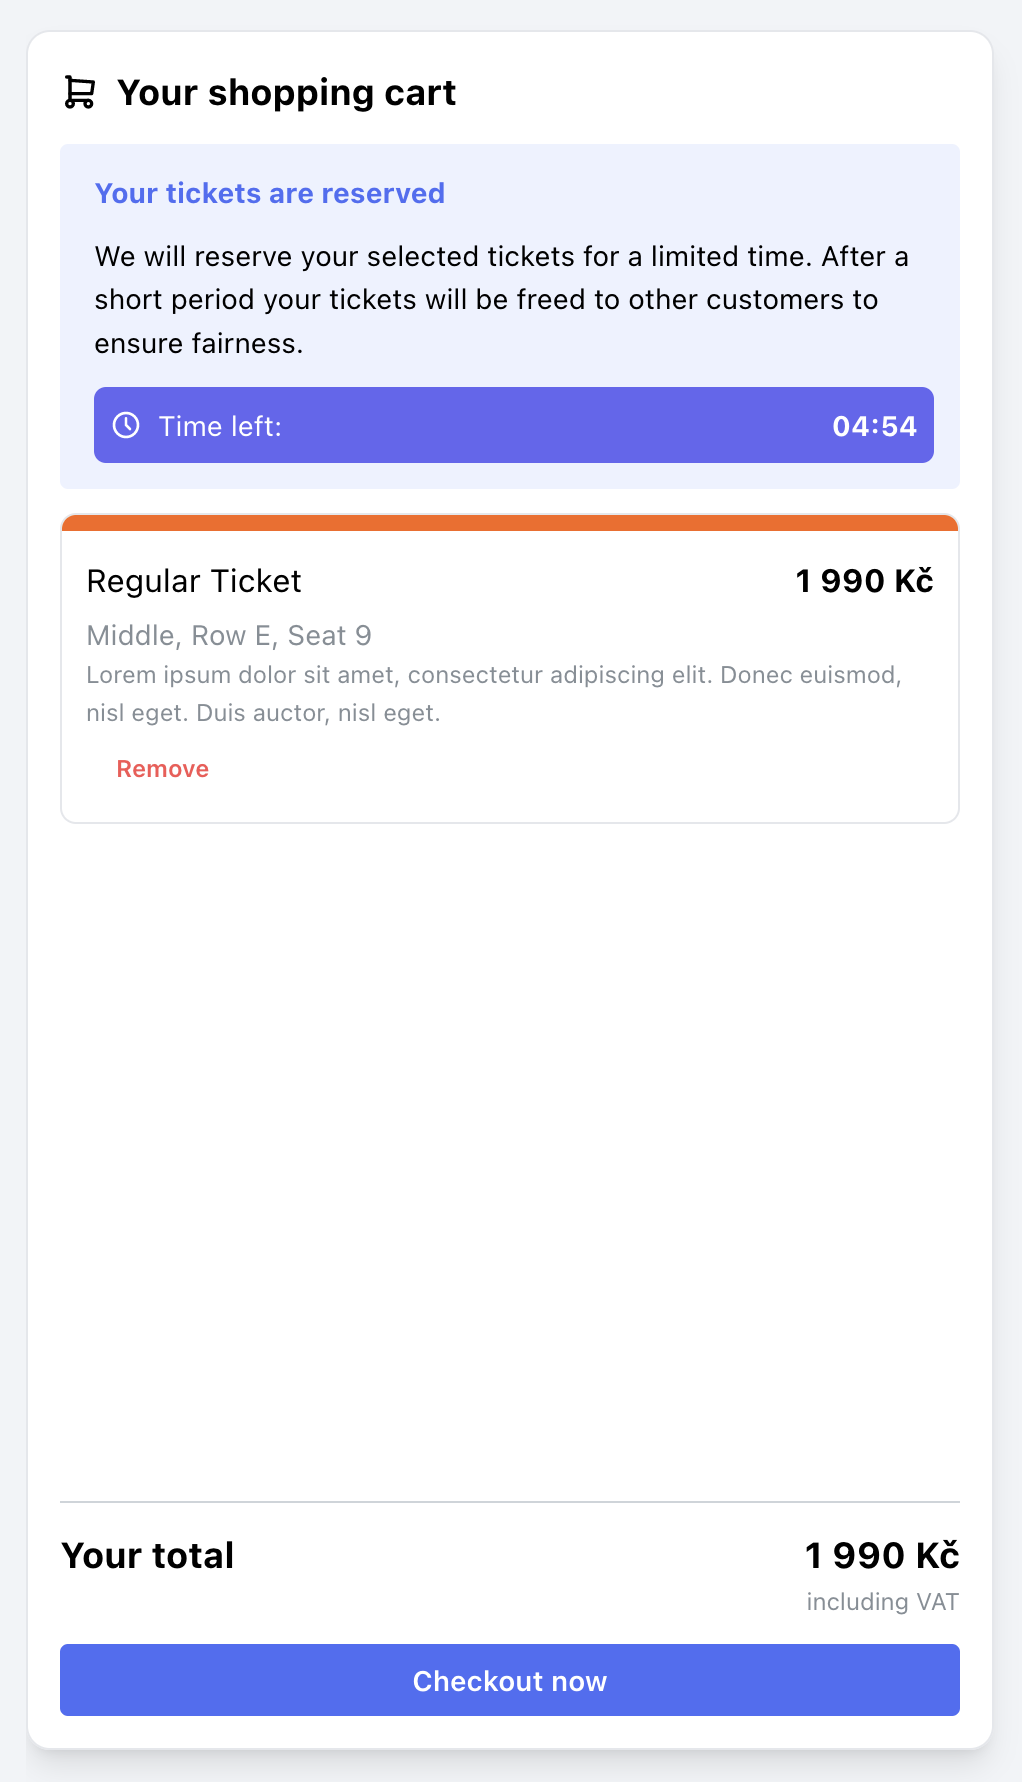
\includegraphics[width=\textwidth]{\FIGDIR/seating-map-reservation-normal}
		\caption{\> 1 min}
		\label{fig:seating-map-reservation-normal}
	\end{subfigure}
	\hfill
	\begin{subfigure}{0.3\textwidth}
		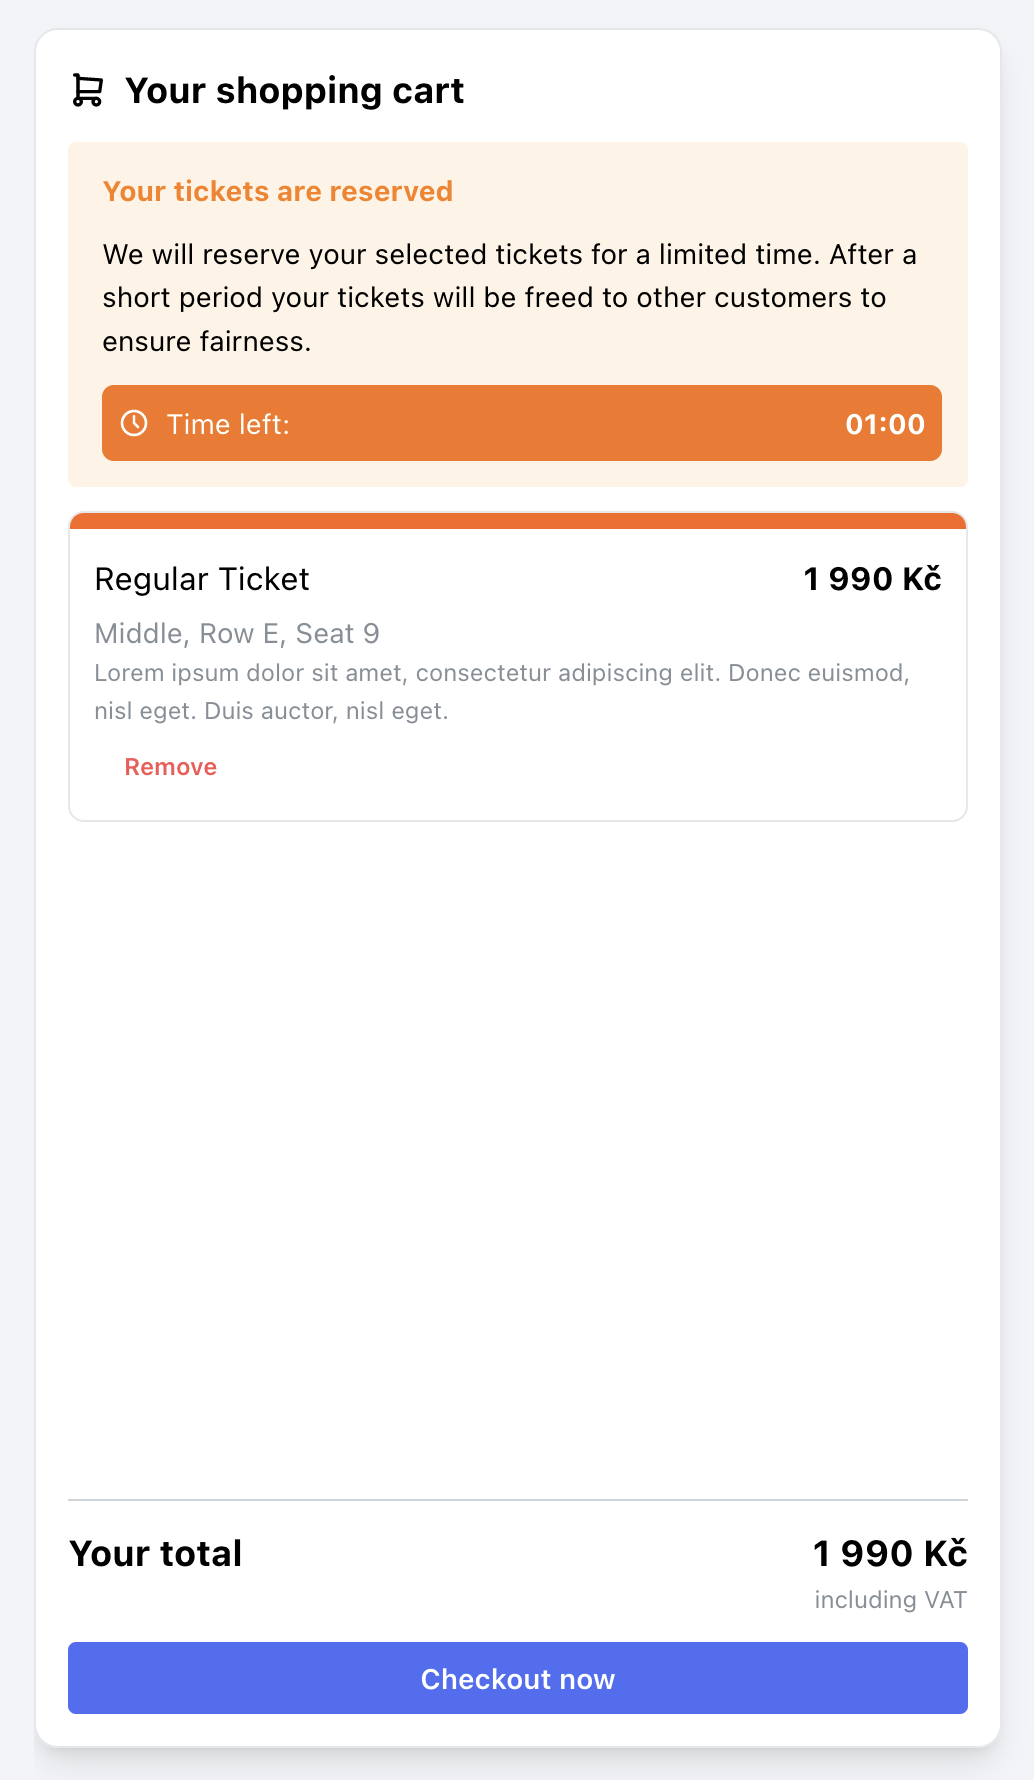
\includegraphics[width=\textwidth]{\FIGDIR/seating-map-reservation-warning}
		\caption{\< 1 min}
		\label{fig:seating-map-reservation-warning}
	\end{subfigure}
	\hfill
	\begin{subfigure}{0.3\textwidth}
		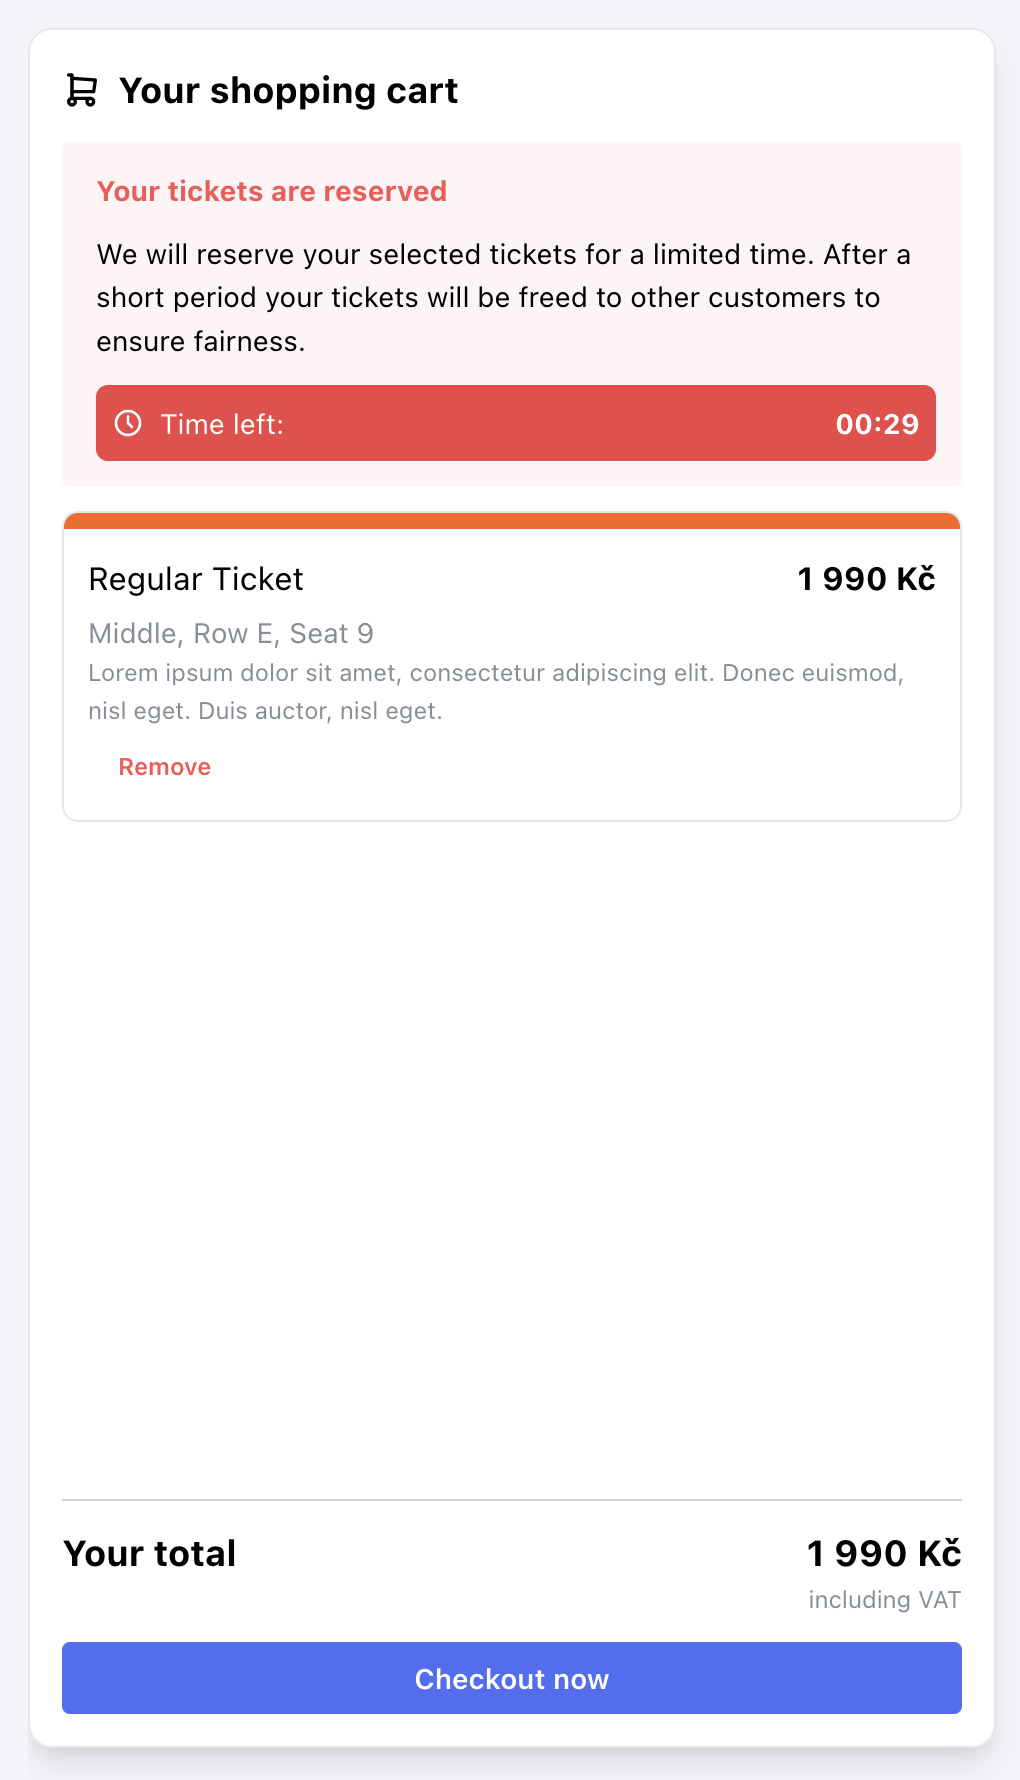
\includegraphics[width=\textwidth]{\FIGDIR/seating-map-reservation-danger}
		\caption{\< 30 s}
		\label{fig:seating-map-reservation-danger}
	\end{subfigure}
	\caption{Upozornění na rezervaci v hlavičce košíku}
	\label{fig:seating-map-reservation}
\end{figure}

Po implementaci rezervačního systému je košík plně funkční.
Další důležitou částí celé implementace je proces objednávky, který je popsán v následující sekci.
